Empezaremos mencionando y caracterizando algunas familias de grafos
para las que nuestra heurist\'ica golosa constructiva siempre encuentra
un resultado correcto, esto es, una clique de m\'axima frontera.

Teniendo en cuenta, como ya se menciono anteriormente, que la heur\'istica
empieza por uno de los nodos de mayor grado y en cada paso va 
agregando nodos que forman clique con los nodos actualmente escogidos
bajo la condici\'on de que el grado de los mismos sea mayor a dos veces
el tama\~no de la clique actual (de estos candidatos, tambi\'en elige
uno de los de mayor grado). Tenemos lo siguiente:

En todos los casos en los que hay varios candidatos para agregar a la
clique con el mismo grado (en particular el primero) la heur\'istica
puede proporcionar el resultado incorrecto, dado que el algoritmo
elige determin\'isticamente uno de los candidatos mientras que la 
entrada es aleatoria (la idea es poder resolver el problema para
cualquier grafo de entrada), veremos a continuaci\'on que excepto
en casos muy particulares, grafos isomorfos cuyas matrices de adyacencia
son distintas pueden, al ser sometidos a la heur\'istica, arrojar
resultados muy dispares (en particular, resultados \'optimos, versus
resultados sub-\'optimos).

\subsubsection{Grafos completos}
	\begin{center}
		\begin{tabular}{ |c||c| }
			\hline
			Grafo de entrada & Paso 1 \\
			\hline\hline
			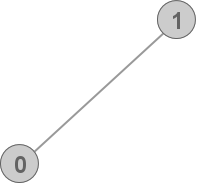
\includegraphics[scale = 0.3]{img/ej3/constructiva_golosa/K2_st0.png} &
			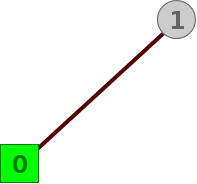
\includegraphics[scale = 0.3]{img/ej3/constructiva_golosa/K2_st1.png} \\
			\hline
			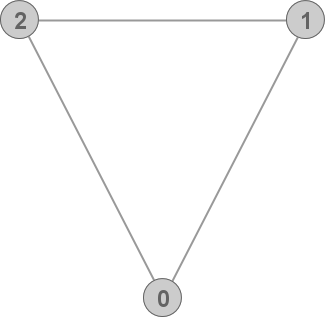
\includegraphics[scale = 0.3]{img/ej3/constructiva_golosa/K3_st0.png} &
			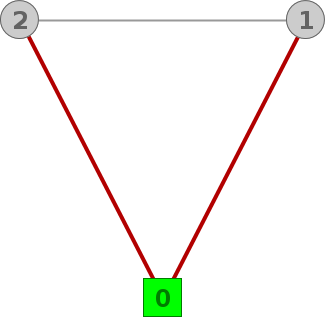
\includegraphics[scale = 0.3]{img/ej3/constructiva_golosa/K3_st1.png} \\
			\hline
		\end{tabular}
		\begin{tabular}{ |c||c||c| }
			\hline
			Grafo de entrada & Paso 1 & Paso 2 \\
			\hline\hline
			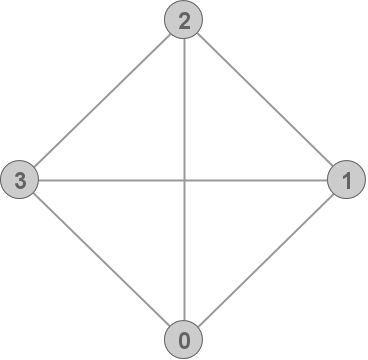
\includegraphics[scale = 0.3]{img/ej3/constructiva_golosa/K4_st0.png} &
			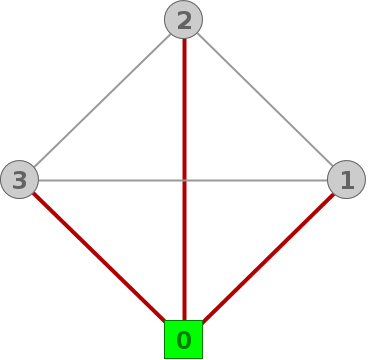
\includegraphics[scale = 0.3]{img/ej3/constructiva_golosa/K4_st1.png} &
			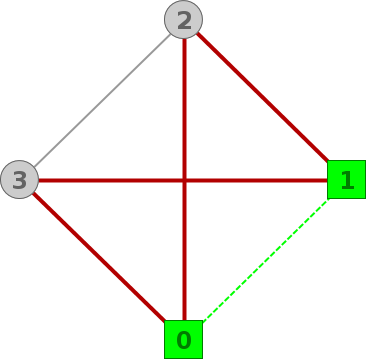
\includegraphics[scale = 0.3]{img/ej3/constructiva_golosa/K4_st2.png} \\
			\hline
			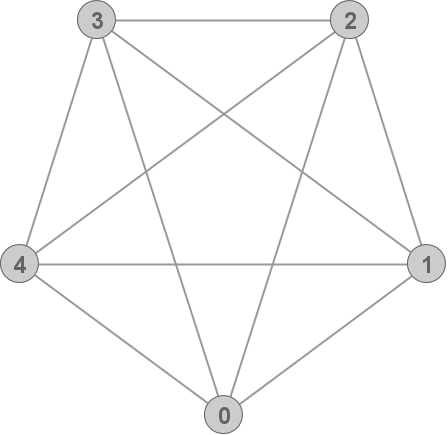
\includegraphics[scale = 0.3]{img/ej3/constructiva_golosa/K5_st0.png} &
			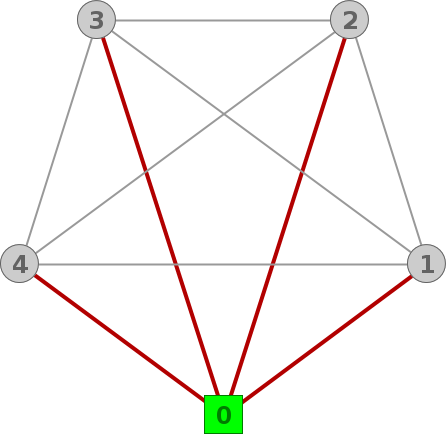
\includegraphics[scale = 0.3]{img/ej3/constructiva_golosa/K5_st1.png} &
			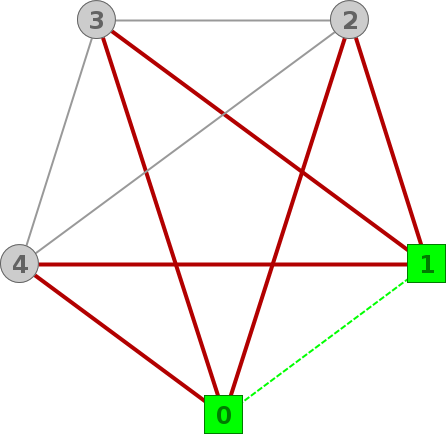
\includegraphics[scale = 0.3]{img/ej3/constructiva_golosa/K5_st2.png} \\
			\hline
		  \end{tabular}
		  \begin{tabular}{ |c||c||c||c| }
			\hline
			Grafo de entrada & Paso 1 & Paso 2 & Paso 3 \\
			\hline\hline
			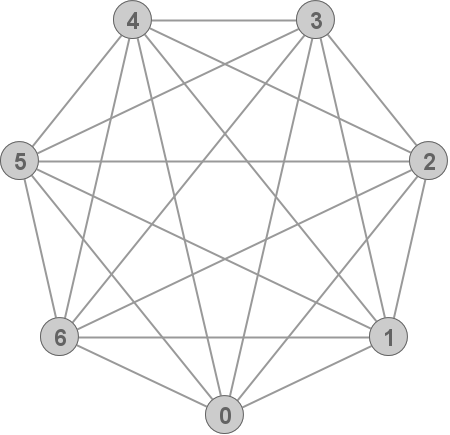
\includegraphics[scale = 0.25]{img/ej3/constructiva_golosa/K7_st0.png} &
			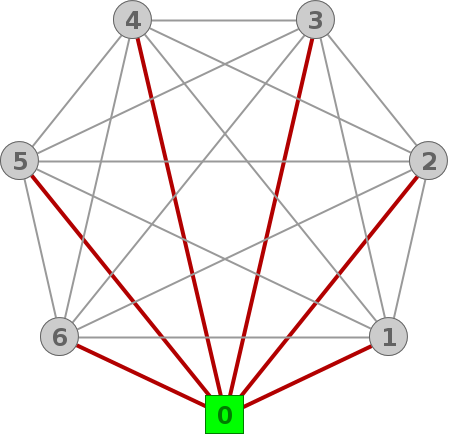
\includegraphics[scale = 0.25]{img/ej3/constructiva_golosa/K7_st1.png} &
			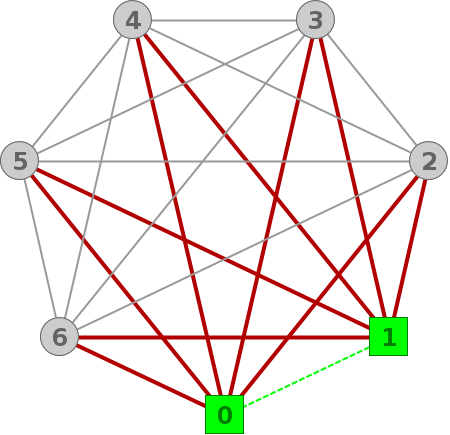
\includegraphics[scale = 0.25]{img/ej3/constructiva_golosa/K7_st2.png} &
			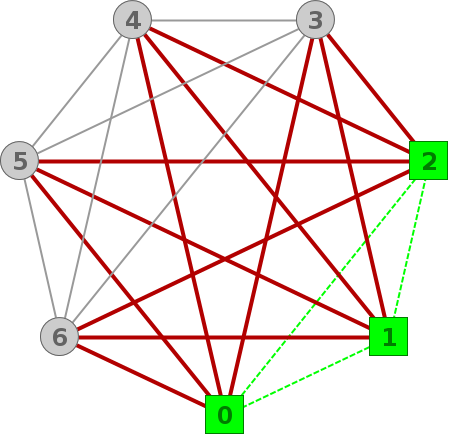
\includegraphics[scale = 0.25]{img/ej3/constructiva_golosa/K7_st3.png} \\
			\hline
		\end{tabular}
	\end{center}

	Todos los algoritmos implementados tienen como uno de sus pasos
	iniciales chequear si el grafo de entrada es un grafo completo, 
	como ya se mencion\'o esto se hace ya que dicho chequeo es $O(1)$
	y la construcci\'on de una $CMF$ toma tiempo $O(n)$, esto si 
	bien no mejora en absoluto la complejidad temporal asint\'otica
	de ninguno de los algoritmos presentados, s\'i permite acortar
	los tiempos de ejecuci\'on lo que sobre un batch de testeo 
	extenso es muy deseable.

	El an\'alisis que se presenta a continuaci\'on es el an\'alisis
	de como se comportar\'ia la heur\'istica de no estar implementada
	esa mejora, se efect\'ua el mismo dado que en familias que 
	veremos m\'as adelante los subgrafos completos juegan un 
	papel importante y su explicaci\'on descansar\'a fuertemente
	sobre las ideas y resultados de este an\'alisis.
	
	Ejemplos de grafos de este tipo y de c\'omo se formar\'ia
	la $CMF$ de no estar implementada la mejora pueden verse
	en el diagrama al principio de esta secci\'on.

	En estos grafos como ya se mencion\'o anteriormente, el algoritmo
	escoger\'ia nodos e ir\'ia haciendo crecer una clique hasta llegar 
	a una 
	clique de tama\~no $n/2$, notes\'e que todos los nodos en los 
	grafos de esta familia tienen grado $d(i) = n - 1$, por lo
	tanto la selecci\'on en cada paso del siguiente nodo de la
	clique ser\'ia dependiente de la implementaci\'on

	Tambi\'en anal\'iticamente puede verse que las CMF para esta 
	familia de grafos son tanto las $K_{\left \lfloor{n/2}\right \rfloor}$ 
	como las $K_{\left \lceil{n/2}\right \rceil}$. Habiendo establecido como
	cota superior al tama\~no de la CMF el valor $n/2$, la posibilidad de que
	los $K_{\left \lceil{n/2}\right \rceil}$ tambi\'en cumplan parece una 
	anomal\'ia a priori. Veremos que no lo es y que est\'a directamente
	relacionado con la naturaleza de la familia en estudio. 

	La frontera es la cantidad de aristas que sale de cada uno de los
	nodos de la clique hacia nodos que no est\'an en la misma. Siendo
	$n$ la cantidad de nodos del grafo y habiendo establecido que la CMF
	tiene tama~no $\left \lfloor{n/2}\right \rfloor$, 
	si la clique en estudio tiene este tama\~no, los nodos que quedan afuera
	de la clique son $\left \lceil{n/2} \right \rceil$, luego: 

	\( 
	\delta(K_{\left \lfloor{n/2}\right \rfloor}) = 
	\left \lfloor{n/2} \right \rfloor \times 
	(n - \left \lfloor{n/2} \right \rfloor ) = 
	\left \lfloor{n/2} \right \rfloor \times 
	(\left \lfloor{n/2} \right \rfloor +
	\left \lceil{n/2} \right \rceil - 
	\left \lfloor{n/2} \right \rfloor) =
	\left \lfloor{n/2} \right \rfloor \times
	\left \lceil{n/2} \right \rceil = 
	\delta(K_{\left \lceil{n/2}\right \rceil})
	\)
%\begin{figure}[H]
%\caption{Ejemplos grafos completos - Entrada / Salida}
%\centering
%%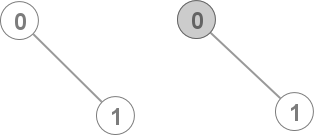
\includegraphics[scale = 0.5]{img/ej3/constructiva_golosa/k2.png}
%%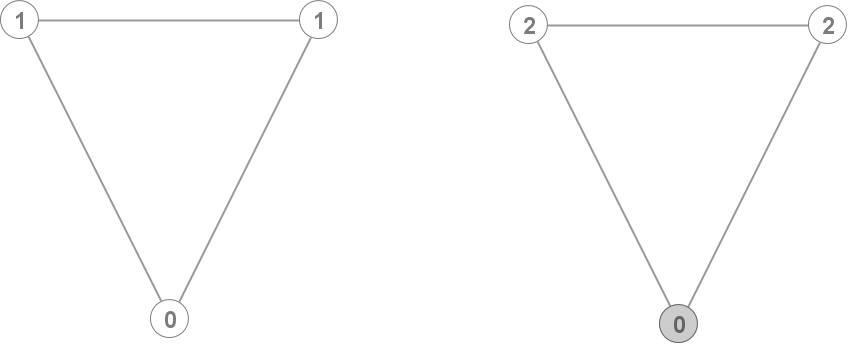
\includegraphics[scale = 0.5]{img/ej3/constructiva_golosa/k3.png}
%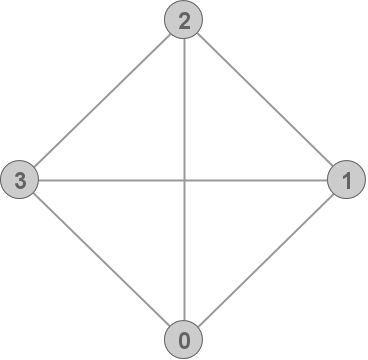
\includegraphics[scale = 0.5]{img/ej3/constructiva_golosa/K4_st0.png}
%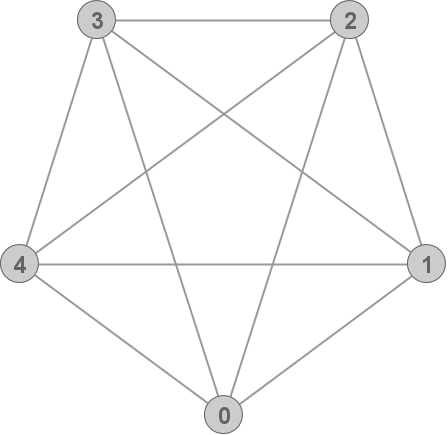
\includegraphics[scale = 0.5]{img/ej3/constructiva_golosa/K5_st0.png}
%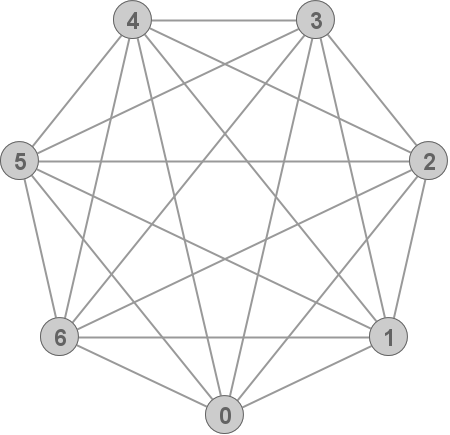
\includegraphics[scale = 0.5]{img/ej3/constructiva_golosa/K7_st0.png}
%\end{figure}

\subsubsection{\'Arboles}
La familia de los \'arboles es una de las familias en las que la heur\'istica
se puede romper y no devolver el resultado correcto. 

Para los \'arboles es pr\'acticamente inmediato que el 
tama\~no de la clique de m\'axima frontera es a lo sumo igual a dos, dado
que por su misma definici\'on los arboles no contienen circuitos simples.

Nuevamente en este caso se toma alguno de los nodos de mayor grado 
y se intenta hacer crecer la clique con alg\'un nodo adyacente.

Como puede verse en los siguientes ejemplos en el caso de que 
implementativamente se seleccione uno de los nodos de mayor grado
adyacente a otro de los nodos de mayor grado, la heur\'istica encuentra
efectivamente una CMF, pero en el caso de que el nodo de partida sea 
uno de los de mayor grado en el grafo y dicho nodo no pertenezca a
ninguna de las CMF del grafo, la heur\'istica reportar\'a un falso 
positivo (una clique cuya frontera es maximal pero no m\'axima).

Desde un punto de vista implementativo el desempate entre nodos de 
mismo grado, depender\'a de la matriz de adyacencia (la posici\'on en
la que aparece un nodo) y dado que existe un arbol isomorfo al del 
ejemplo en el que el nodo incorrecto para empezar la clique est\'a
listado antes que el nodo correcto (el que permite generar la CMF),
el siguiente es un buen ejemplo para ilustrar la fragilidad de la
heur\'istica

%\begin{figure}[H]
%\caption{Ejemplos \'Arboles}
%\centering
%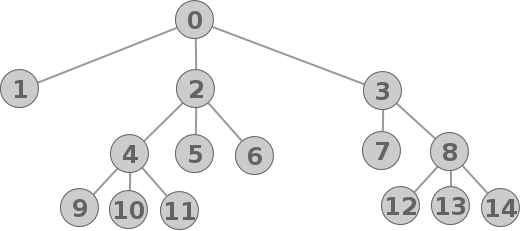
\includegraphics[scale = 0.5]{img/ej3/constructiva_golosa/tree_st0.png}
%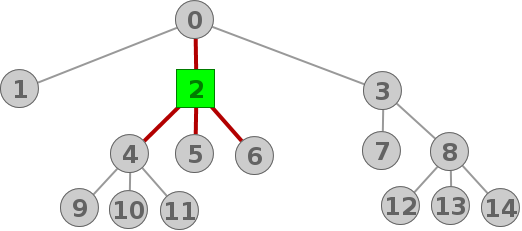
\includegraphics[scale = 0.5]{img/ej3/constructiva_golosa/tree_st01.png}
%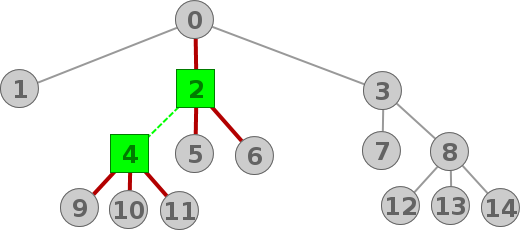
\includegraphics[scale = 0.5]{img/ej3/constructiva_golosa/tree_st02.png}
%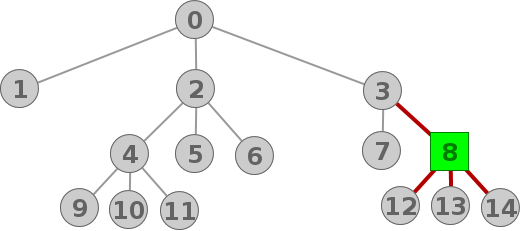
\includegraphics[scale = 0.5]{img/ej3/constructiva_golosa/tree_st11.png}
%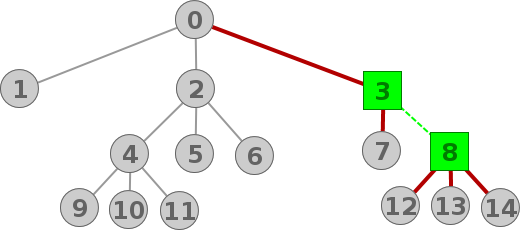
\includegraphics[scale = 0.5]{img/ej3/constructiva_golosa/tree_st12.png}
%\end{figure}

	\begin{center}
		\begin{tabular}{ |c||c||c| }
			\hline
			Grafo de entrada & Paso 1 & Paso2 \\
			\hline\hline
			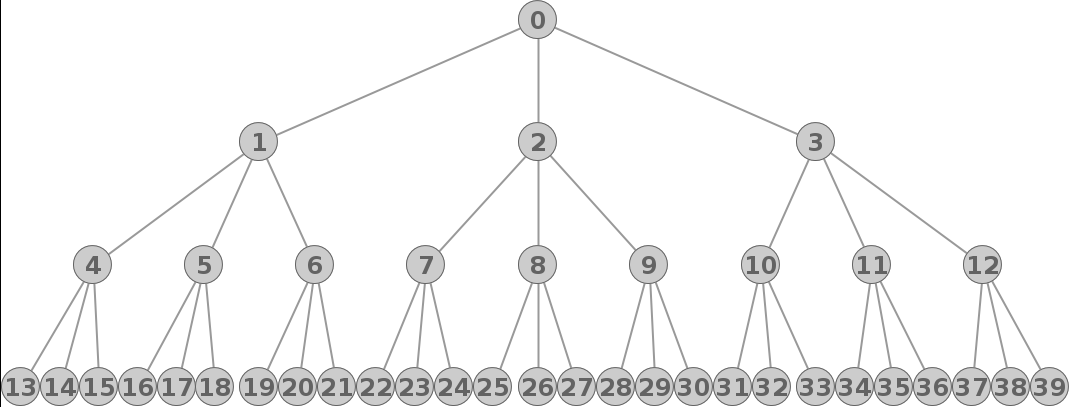
\includegraphics[scale = 0.15]{img/ej3/constructiva_golosa/ctree_st0.png} &
			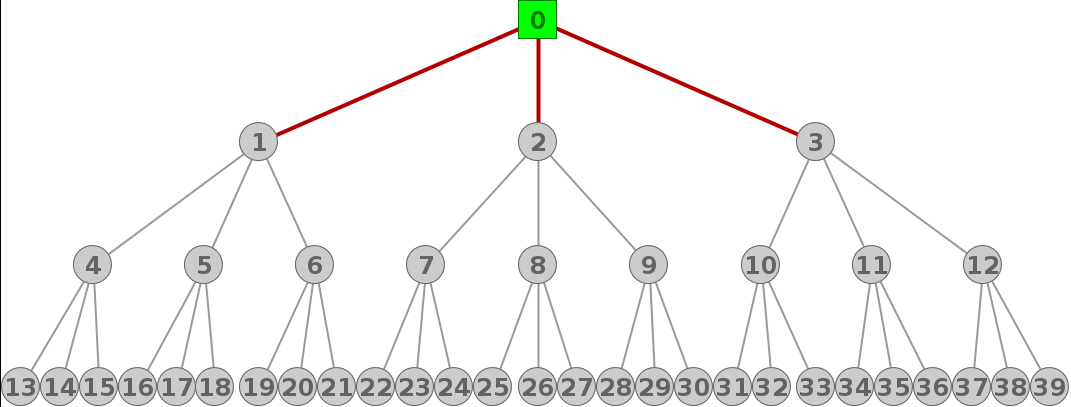
\includegraphics[scale = 0.15]{img/ej3/constructiva_golosa/ctree_st1.png} &
			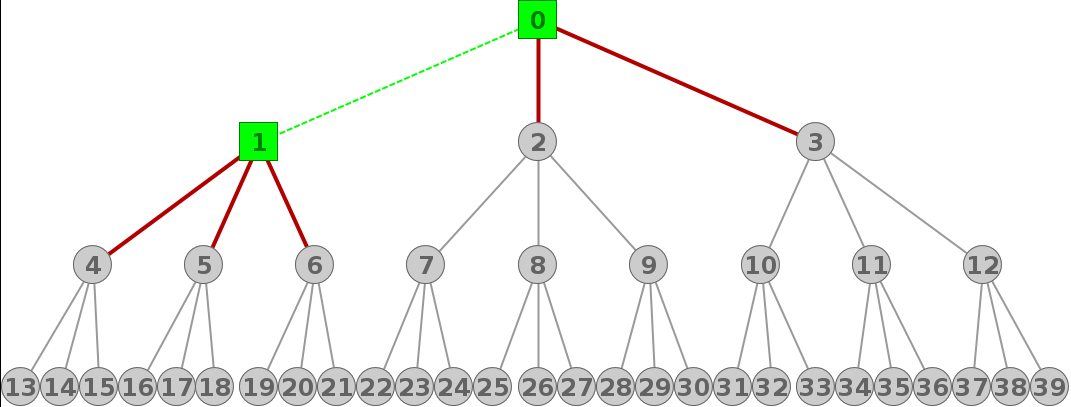
\includegraphics[scale = 0.15]{img/ej3/constructiva_golosa/ctree_st2.png} \\
			\hline
			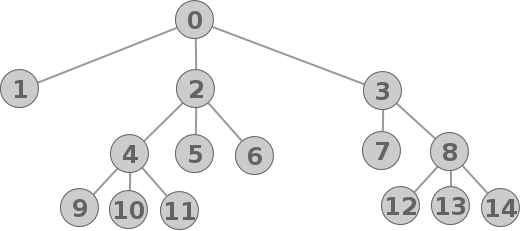
\includegraphics[scale = 0.3]{img/ej3/constructiva_golosa/tree_st0.png} &
			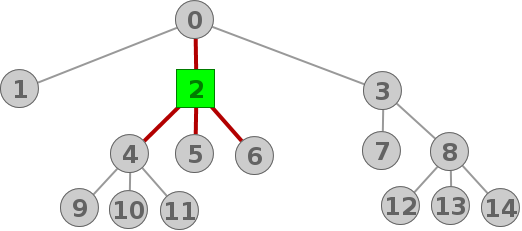
\includegraphics[scale = 0.3]{img/ej3/constructiva_golosa/tree_st01.png} &
			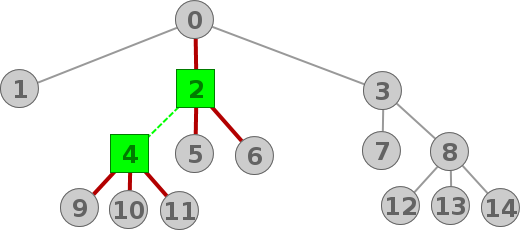
\includegraphics[scale = 0.3]{img/ej3/constructiva_golosa/tree_st02.png} \\
			\hline
			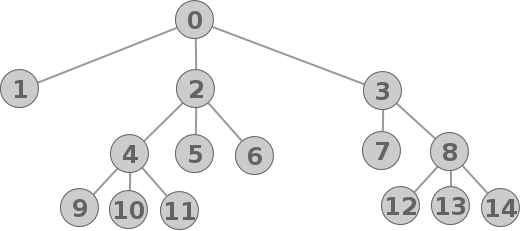
\includegraphics[scale = 0.3]{img/ej3/constructiva_golosa/tree_st0.png} &
			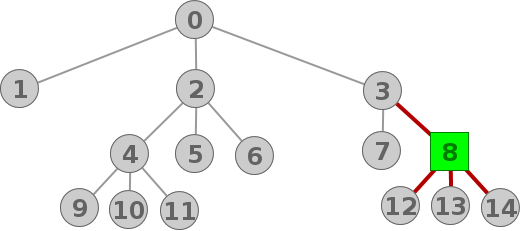
\includegraphics[scale = 0.3]{img/ej3/constructiva_golosa/tree_st11.png} &
			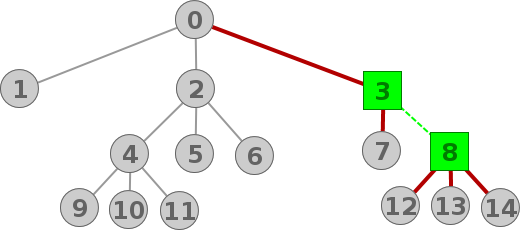
\includegraphics[scale = 0.3]{img/ej3/constructiva_golosa/tree_st12.png} \\
			\hline
		\end{tabular}
	\end{center}

An\'alizando lo mucho que se puede apartar la soluci\'on \'optima de una soluci\'on sub-\'optima
podemos ver que si llamamos $v$ al nodo de mayor grado en el arbol y tomamos $d(v) = \Delta$, la
mayor frontera que puede tener la $CMF$ (o sea la soluci\'on \'optima) es
\[ \delta(CMF) = \Delta -1 + \Delta -1 = 2 \Delta -2 \]
esto sucede cuando $v$ (el primer nodo elegido por el algoritmo) es adyacente a otro nodo de grado
$\Delta$ ($v'$ en el gr\'afico). Mientras que la soluci\'on menos \'optima que se puede obtener es 
cuando el nodo de mayor grado adyacente a $v$ es de grado menor a 3 
(de este modo, la clique calculada no crece del nodo original) dandonos una soluci\'on sub-\'optima
\[ \delta(SH) = \Delta \]

	\begin{figure}[H]
	\caption{Un ejemplo extremo para \'arboles}
	\label{fig:extremo_arboles}
	\begin{center}
		\begin{tabular}{|c||c||c||c|}
		\hline
		& Grafo de entrada & Paso 1 & Paso 2 \\ 
			\hline
			resultado sub-\'optimo &
			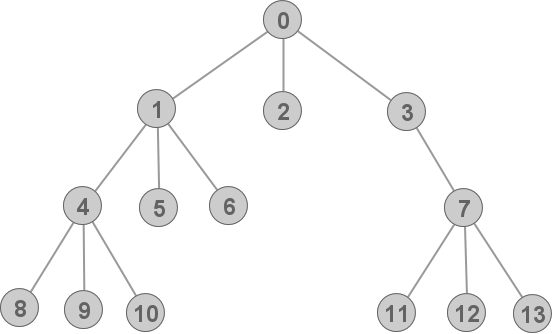
\includegraphics[scale = 0.2]{img/ej3/constructiva_golosa/extremetree_st0.png} &
			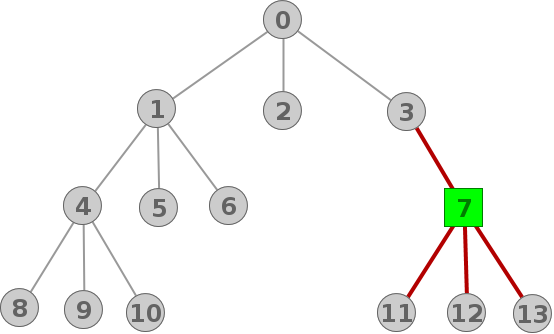
\includegraphics[scale = 0.2]{img/ej3/constructiva_golosa/extremetree_st11.png} & \\
			\hline
			resultado \'optimo &
			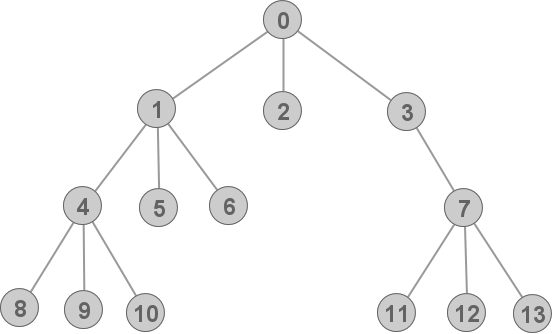
\includegraphics[scale = 0.2]{img/ej3/constructiva_golosa/extremetree_st0.png} &
			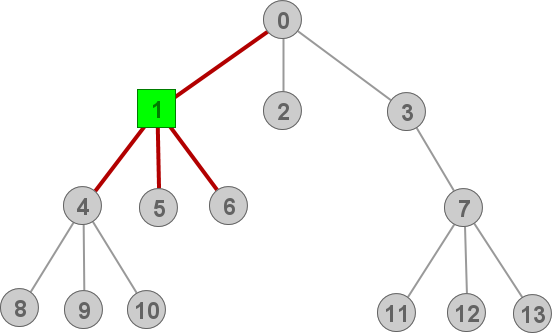
\includegraphics[scale = 0.2]{img/ej3/constructiva_golosa/extremetree_st01.png} & 
			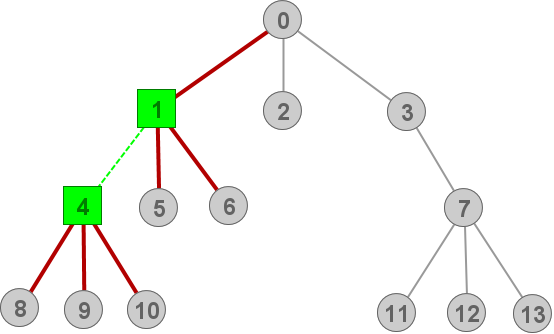
\includegraphics[scale = 0.2]{img/ej3/constructiva_golosa/extremetree_st02.png} \\
		\hline
		\end{tabular}
	\end{center}
	\end{figure}
	
Con esto se puede ver que la soluci\'on calculada por la heur\'istica ($\delta(SH)$) es $O(\Delta)$ 
y la soluci\'on \'optima ($\delta(CMF)$) tambi\'en es $O(\Delta)$ con lo que la raz\'on entre ambas 
es constante.
			
\subsubsection{Grafos bipartitos}
\label{subsub:bipartitos}
	Para los grafos bipartitos tenemos un problema similar que el que tenemos para los \'arboles.
	Cuando el grafo es bipartito completo al tener todos los nodos de cada una de las particiones
	el mismo grado, la heur\'istica funciona bien. Cuando esto no pasa, puede suceder que la 
	heur\'istica produzca el resultado \'optimo como tambi\'en que produzca un resultado sub-\'optimo.
	Esta situaci\'on puede verse en el \'ultimo ejemplo mostrado m\'as abajo, ambos resultados pueden
	ser arrojados por el algoritmo dependiendo de la implementaci\'on. 
	

	\begin{center}
		\begin{tabular}{ |c||c||c| }
			\hline
			Grafo de entrada & Paso 1 & Paso2 \\
			\hline\hline
			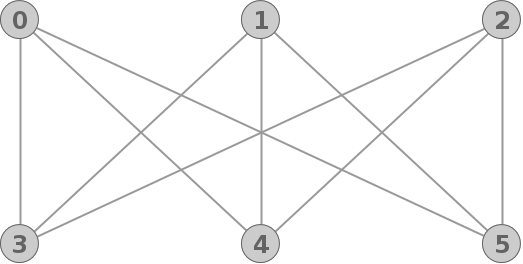
\includegraphics[scale = 0.2]{img/ej3/constructiva_golosa/k3,3_st0.png} &
			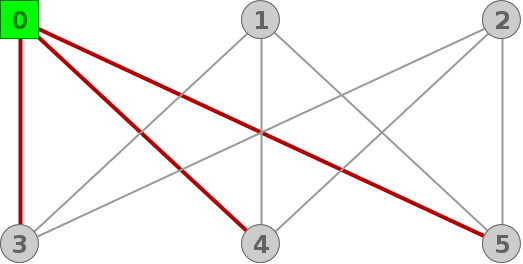
\includegraphics[scale = 0.2]{img/ej3/constructiva_golosa/k3,3_st1.png} &
			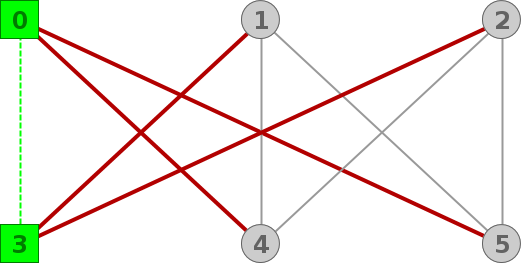
\includegraphics[scale = 0.2]{img/ej3/constructiva_golosa/k3,3_st2.png} \\
			\hline
			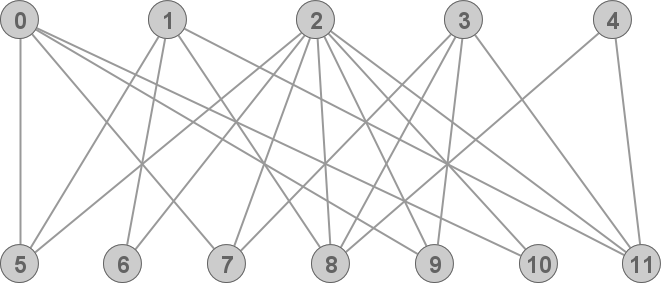
\includegraphics[scale = 0.2]{img/ej3/constructiva_golosa/bipartito1_st0.png} &
			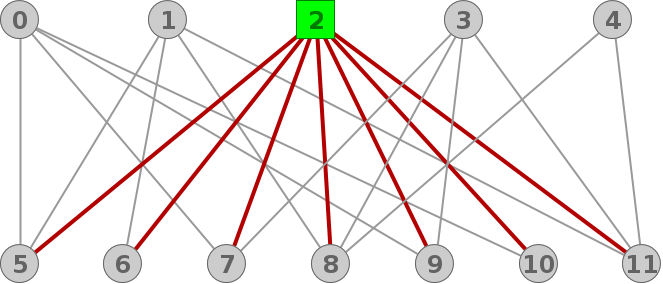
\includegraphics[scale = 0.2]{img/ej3/constructiva_golosa/bipartito1_st01.png} &
			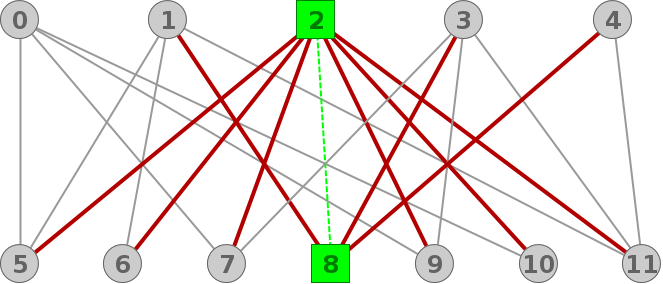
\includegraphics[scale = 0.2]{img/ej3/constructiva_golosa/bipartito1_st02.png} \\
			\hline
		\end{tabular}
	\end{center}
	\begin{center}
		\begin{tabular}{ |c||c||c||c| }
		\hline
		& Grafo de entrada & Paso 1 & Paso2 \\
		\hline\hline
		resultado sub-\'optimo & 
		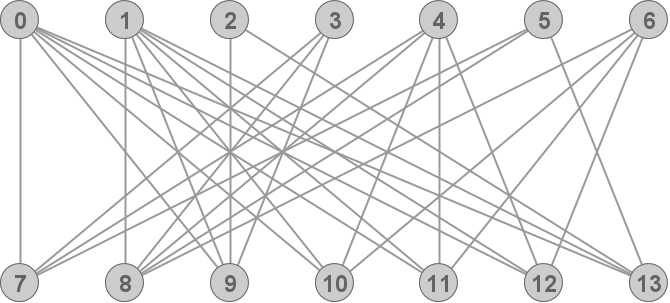
\includegraphics[scale = 0.18]{img/ej3/constructiva_golosa/bipartito2_st0.png} &
		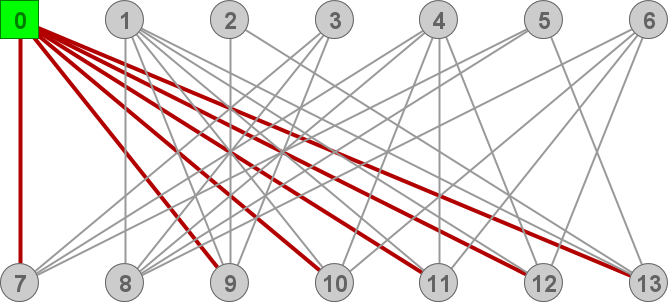
\includegraphics[scale = 0.18]{img/ej3/constructiva_golosa/bipartito2_st01.png} &
		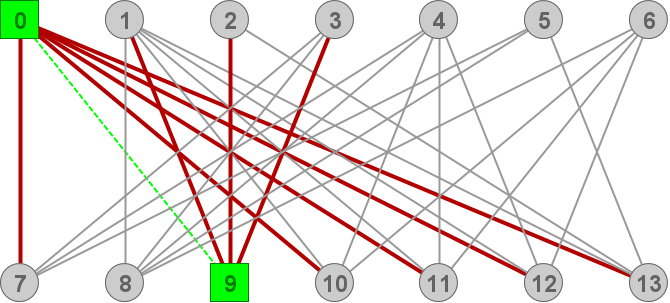
\includegraphics[scale = 0.18]{img/ej3/constructiva_golosa/bipartito2_st02.png} \\
		\hline
		resultado \'optimo&
		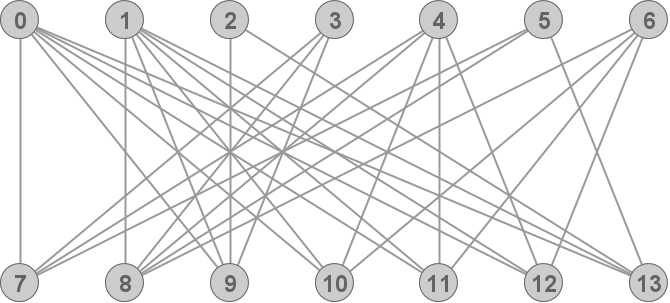
\includegraphics[scale = 0.18]{img/ej3/constructiva_golosa/bipartito2_st0.png} &
		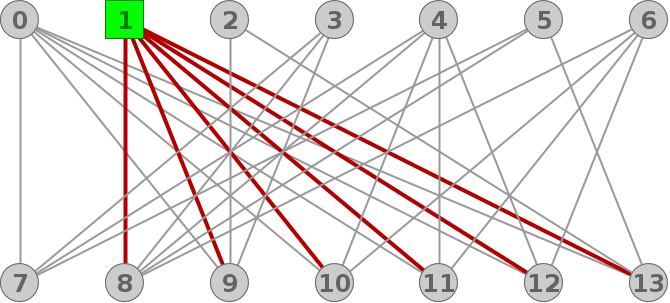
\includegraphics[scale = 0.18]{img/ej3/constructiva_golosa/bipartito2_st11.png} &
		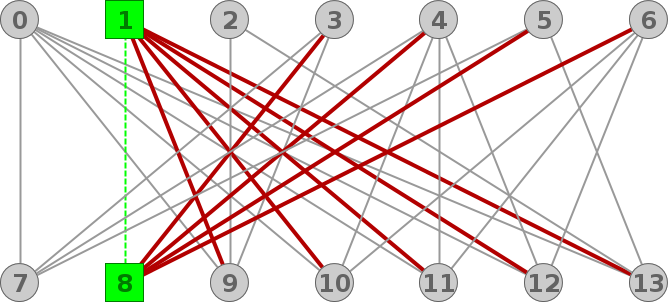
\includegraphics[scale = 0.18]{img/ej3/constructiva_golosa/bipartito2_st12.png} \\
		\hline
		\end{tabular}
	\end{center}
	
	Para construir un ejemplo extremo 
	en el que se rompe el funcionamiento de la heur\'istica se parte de la idea de tener dos nodos
	de grado m\'aximo $\Delta$, uno de los cuales est\'a conectado con todos los nodos de la otra
	partici\'on excepto con un nodo distinguido, todos los nodos de la otra partici\'on tendr\'an
	grado $\leq 2$ excepto el nodo distinguido que tendr\'a grado $\Delta -1$, el otro nodo de grado
	m\'aximo estar\'a conectado con todos los nodos de la partici\'on opuesta, excepto con alguno
	que no sea el nodo distinguido. Los nodos restantes de la partici\'on que contiene a los de 
	grado m\'aximo solo estar\'an conectados con el nodo distinguido de la partici\'on contraria.

	\begin{figure}[H]
	\caption{Un ejemplo extremo para bipartitos}
	\label{fig:extremo_bipartito}
	\begin{center}
		\begin{tabular}{|c||c||c||c|}
		\hline
		& Grafo de entrada & Paso 1 & Paso 2 \\ 
			\hline
			resultado sub-\'optimo &
			\includegraphics[scale = 0.2]{img/ej3/constructiva_golosa/k5,4Nocompleto_st0.png} &
			\includegraphics[scale = 0.2]{img/ej3/constructiva_golosa/k5,4Nocompleto_st01.png} & \\
			\hline
			resultado \'optimo &
			\includegraphics[scale = 0.2]{img/ej3/constructiva_golosa/k5,4Nocompleto_st0.png} &
			\includegraphics[scale = 0.2]{img/ej3/constructiva_golosa/k5,4Nocompleto_st11.png} & 
			\includegraphics[scale = 0.2]{img/ej3/constructiva_golosa/k5,4Nocompleto_st12.png} \\
		\hline
		\end{tabular}
	\end{center}
	\end{figure}

	Aqu\'i se puede ver que por construcci\'on, si llamamos a los nodos de grado m\'aximo en el grafo
	$v$ y $v'$, definimos $d(v) = d(v') = \Delta$ y llamamos al nodo distinguido de la partici\'on
	alternativa $x$, con $v$ no adyacente a $x$, tenemos que $d(x) = \Delta -1$. 
	Si luego asumimos que la estructura del grafo de entrada viene ordenada de forma tal que la 
	heur\'istica seleccione como primer nodo de la clique al nodo $v$, tenemos la frontera
	devuelta por la heur\'istica ($\delta(SH)$)
	\[\delta(SH) = \Delta -1 \]
	y la frontera de la $CMF$
	\[\delta(CMF) = 2 \Delta -3 \]

	Con esto, haciendo abuso de notacion tenemos $\delta(SH) = O(\Delta)$ y $\delta(CMF) = O(\Delta)$ con 
	lo que nuevamente la raz\'on entre entre ambas es constante.

\subsubsection{Grafos circulares}
\label{subsub:circulares}
	En este tipo de grafos, si bien nos encontramos con el problema de empate en el 
	grado de los nodos, tenemos la ventaja (como la ten\'iamos para los grafos completos)
	que el grado de todos los nodos es el mismo, con lo cual tenemos asegurado que 
	nuestra heur\'istica arrojar\'a resultados \'optimos.
	\begin{center}
		\begin{tabular}{ |c||c| }
			\hline
			Grafo de entrada & Paso 1 \\
			\hline\hline
			\includegraphics[scale = 0.4]{img/ej3/constructiva_golosa/Circle_st0.png} &
			\includegraphics[scale = 0.4]{img/ej3/constructiva_golosa/Circle_st1.png} \\
			\hline
		\end{tabular}
	\end{center}

\subsubsection{Estrellas/Ruedas}
\label{subsub:ruedas}
	Para esta familia nos encontramos con el problema del empate en el grado cuando 
	el algoritmo llega a la selecci\'on del segundo nodo para formar la $CMF$, aqu\'i
	tambi\'en el alto grado de simetr\'ia radial de esta famil\'ia viene en nuestra 
	ayuda, puesto que al compartir todos los nodos (excepto el central) el mismo grado
	es indistinto cual se elige, arrojando el mismo resultado independientemente del 
	proceso de selecci\'on, con lo cual nuestra heur\'istica funciona correctamente
	en todos los casos. En el caso de la estrella adicionalmente, nunca se elige un 
	segundo nodo.

	\begin{center}
		\begin{tabular}{ |c||c| }
			\hline
			Grafo de entrada & Paso 1 \\
			\hline\hline
			\includegraphics[scale = 0.25]{img/ej3/constructiva_golosa/Star_st0.png} &
			\includegraphics[scale = 0.25]{img/ej3/constructiva_golosa/Star_st1.png} \\
			\hline
		 \end{tabular}
		 \begin{tabular}{ |c||c||c| }
			\hline
			Grafo de entrada & Paso 1 & Paso 2 \\
			\hline\hline
			\includegraphics[scale = 0.25]{img/ej3/constructiva_golosa/Wheel_st0.png} &
			\includegraphics[scale = 0.25]{img/ej3/constructiva_golosa/Wheel_st1.png} &
			\includegraphics[scale = 0.25]{img/ej3/constructiva_golosa/Wheel_st2.png} \\
			\hline
		\end{tabular}
	\end{center}

\subsubsection{Banana tree}
\label{subsub:banana}
	Para est\'a familia tambi\'en nos encontramos con un caso de empate entre todos los 
	nodos seleccionables (cuando el nodo de lo que ser\'ia la ra\'iz en caso de ser
	un \'arbol dirigido es uno de los nodos de mayor grafo), o en el caso de que
	haya siempre un \'unico candidato que cumpla con la exigencia de que su grado sea
	mayor a dos veces el tama\~no de la clique actual. Esto es debido a la estricta 
	caracterizaci\'on de esta familia de grafos. Aqu\'i tambi\'en el algoritmo 
	devolver\'a la soluci\'on \'optima.
	\begin{center}
		\begin{tabular}{ |c||c|c| }
			\hline
			Grafo de entrada & Paso 1 & Paso 2 \\
			\hline\hline
			\includegraphics[scale = 0.2]{img/ej3/constructiva_golosa/banana4,4_st0.png} &
			\includegraphics[scale = 0.2]{img/ej3/constructiva_golosa/banana4,4_st1.png} & 
			\includegraphics[scale = 0.2]{img/ej3/constructiva_golosa/banana4,4_st2.png} \\
			\hline
			\includegraphics[scale = 0.2]{img/ej3/constructiva_golosa/banana5,7_st0.png} &
			\includegraphics[scale = 0.2]{img/ej3/constructiva_golosa/banana5,7_st1.png} &
			\includegraphics[scale = 0.2]{img/ej3/constructiva_golosa/banana5,7_st2.png} \\
			\hline
		\end{tabular}
	\end{center}




%La familia de gr\'afos que asegura un resultado incorrecto de nuestra 
%heur\'istica golosa puede ser caracterizada como aquella en la que el
%nodo de mayor grado no forma parte de la clique de m\'axima frontera.
%Esto sucede ya que la heur\'istica construye una clique a partir del 
%nodo de grado m\'aximo y en cada paso se mantiene el invariante de 
%de clique, agregando solamente nodos cuyo grado sea mayor al tama\~no
%de la clique en ese paso, por lo tanto si alguno de los nodos de la 
%clique de m\'axima frontera no forma clique con el nodo 
%inicial (el de mayor grado) entonces la heuristica constructiva no 
%puede llegar a incluir a ese nodo.
%
%Ejemplos:
%
%%\begin{tikzpicture}
%%	\SetGraphUnit{1.5cm}
%%	\GraphInit[vstyle=Normal]
%%
%%	\Vertices{circle}{2,5,6,7,8}
%%	\WE(2){1}
%%	\Vertices{circle}{3,10,9,11}
%%	\WE(3){2}
%%
%%	\foreach \v in {2,5,6,7,8}{\Edge(1)(\v)};
%%
%%\end{tikzpicture}
%	
%\begin{tikzpicture}
%	\path 	
%			% Nodos
%			(0,8) node [shape=circle, draw] (1) {1}
%			(1,8) node [shape=circle, draw] (2) {2}
%			(2,8) node [shape=circle, draw] (3) {3}
%			(6,8) node [shape=circle, draw] (4) {4}
%			(7,8) node [shape=circle, draw] (5) {5}
%			(8,8) node [shape=circle, draw] (6) {6}
%			(0,7) node [shape=circle, draw] (7) {7}
%			(1,7) node [shape=circle, draw] (8) {8}
%			(7,7) node [shape=circle, draw] (9) {9}
%			(8,7) node [shape=circle, draw] (10) {10}
%			(0,6) node [shape=circle, draw] (11) {11}
%			(1,6) node [shape=circle, draw] (12) {12}
%			(7,6) node [shape=circle, draw] (13) {13}
%			(8,6) node [shape=circle, draw] (14) {14}
%			(4,5) node [shape=circle, draw] (15) {15}
%			(2,4) node [shape=circle, draw] (16) {16}
%			(3,4) node [shape=circle, draw] (17) {17}
%			(5,4) node [shape=circle, draw] (18) {18}
%			(6,4) node [shape=circle, draw] (19) {19}
%			(2,3) node [shape=circle, draw] (20) {20}
%			(3,3) node [shape=circle, draw] (21) {21}
%			(4,3) node [shape=circle, draw] (22) {22}
%			(5,3) node [shape=circle, draw] (23) {23}
%			(6,3) node [shape=circle, draw] (24) {24}
%			(2,2) node [shape=circle, draw] (25) {25}
%			(6,2) node [shape=circle, draw] (26) {26}
%			(4, 1.5) node [shape=circle, draw] (27) {27}
%			(2,1) node [shape=circle, draw] (28) {28}
%			(6,1) node [shape=circle, draw] (29) {29}
%			(2,0) node [shape=circle, draw] (30) {30}
%			(3,0) node [shape=circle, draw] (31) {31}
%			(5,0) node [shape=circle, draw] (32) {32}
%			(6,0) node [shape=circle, draw] (33) {33};
%			% Aristas de la semiestrella superior izq
%			\draw[-] (1) -- (8);
%			\draw[-] (2) -- (8);
%			\draw[-] (3) -- (8);
%			\draw[-] (7) -- (8);
%			\draw[-] (11) -- (8);
%			\draw[-] (12) -- (8);
%
%			% Aristas de la semiestrella superior izq
%			\draw[-] (4) -- (9);
%			\draw[-] (5) -- (9);
%			\draw[-] (6) -- (9);
%			\draw[-] (10) -- (9);
%			\draw[-] (13) -- (9);
%			\draw[-] (14) -- (9);
%
%			% Mas aristas
%			
%			\draw[-] (8) -- (9);
%			\draw[-] (8) -- (15);
%			\draw[-] (9) -- (15);
%			\draw[-] (16) -- (15);
%			\draw[-] (17) -- (15);
%			\draw[-] (18) -- (15);
%			\draw[-] (19) -- (15);
%			\draw[-] (22) -- (15);
%
%			% Aristas de la estrella inferior
%
%			\draw[-] (20) -- (27);
%			\draw[-] (21) -- (27);
%			\draw[-] (22) -- (27);
%			\draw[-] (23) -- (27);
%			\draw[-] (24) -- (27);
%			\draw[-] (25) -- (27);
%			\draw[-] (26) -- (27);
%			\draw[-] (28) -- (27);
%			\draw[-] (29) -- (27);
%			\draw[-] (30) -- (27);
%			\draw[-] (31) -- (27);
%			\draw[-] (32) -- (27);
%			\draw[-] (33) -- (27);
%
%			
%\end{tikzpicture}

\subsection{Construcci\'on de familias que rompen siempre la heur\'istica}

Intentando construir familias que siempre van a romper la heur\'istica llegamos a las siguientes
(en lo siguiente llamaremos $v$ al \'unico nodo de grado m\'aximo en un grafo):
\begin{itemize}
	\item{$v \notin CMF$}
	\item{$v \in CMF$}
\end{itemize}

Por construcci\'on estaremos viendo familias en las que existe un \'unico nodo de grado m\'aximo en el grafo.

Construyamos la primera familia que rompe la heur\'istica

\subsubsection{Estrella + Puente + CMF ($v$ no en $CMF$)}

Estamos buscando una familia de grafos en los que el nodo de grado m\'aximo no forme parte de la 
frontera, con esto en mente, partimos de un nodo de grado m\'aximo: $v$, para lograr esto $v$ ser\'a
en un principio el nodo central de una estrella. Con este escenario si la $CMF$ contuviera a $v$, la
$CMF$ ser\'ia la clique formada \'unicamente por $v$ (m\'as adelante estudiaremos como nos afecta 
relajar esta condici\'on). Como estamos viendo el caso en el que no pertenece, necesitamos una clique 
que por comodidad en un principio generaremos desconectada de $v$ para luego conectarla por 
intermedio de un puente, esto es, un camino simple entre uno de los nodos de la estrella (cualquiera
excepto $v$) y uno de los nodos de la clique al que llamaremos $v'$. 

La idea es que la $CMF$ sea parte de esa clique que agregamos, utilizamos el puente para asegurarnos
de que debido a la naturaleza de nuestra heur\'istica, esta no pueda construir una clique que contenga
a $v$ y a $v'$.

Llamemos $\Delta$ al grado de $v$, o sea la estrella tendr\'a $\Delta$ puntas. Con nuestra construcci\'on 
$v'$ puede tener a lo sumo grado $\Delta -1$, adicionalmente $v'$ es parte de una clique que luego ser\'a 
conectada por un puente a la estrella con lo que una de las aristas de $v'$ ser\'a parte del puente. 
Con esto la clique podr\'a tener a lo sumo tama\~no $\Delta -1$, dado que el grado de cada uno de los 
nodos de la clique entonces ser\'a $\Delta -2$, asegurando entonces que el grado de $v'$ no excede
el l\'imite impuesto, siempre y cuando $v'$ no tenga aristas adicionales a las que lo hacen 
parte de la clique, excepto la que lo conecta al puente.

Gr\'aficamente:
\begin{figure}[H]
\caption{Estrella + Puente + CMF}
\label{fig:epcmf_carac}
\begin{center} 
	\includegraphics[scale = 0.6]{img/ej3/constructiva_golosa/vnotincmf_carac1.png} 
\end{center}
\end{figure}

Ahora analicemos cual es la frontera de la $CMF$: $\delta (CMF)$

Como vimos anteriormente, sabemos que la $CMF$ dentro de una clique $K_k$ tiene tama\~no
$\left\lfloor \frac{k}{2} \right \rfloor$. Tambi\'en en este caso nuestra $CMF$ deber\'a
contener a $v'$ ya que este nodo agrega una arista extra a la frontera que se puede conseguir
de cualquier clique que no lo contenga.

La frontera de esta $CMF$ asi caracterizada se calcula como la cantidad de nodos de la $CMF$
multiplicada por la cantidad de aristas que la conectan con el resto de los nodos, en este caso
(teniendo en cuenta la arista extra que conecta $v'$ con el puente):

\[ \delta(CMF) = (\left\lfloor \frac{\Delta -1}{2} \right\rfloor) \times 
	(\left\lceil \frac{\Delta -1}{2} \right\rceil) + 1 \]

Separamos en dos casos, si $\Delta$ es impar, $\Delta -1$ es par y tenemos
\[ \boxed{\delta(CMF) = (\frac{\Delta -1}{2})^2 +1} \text{ Con $\Delta$ impar} \]

si $\Delta$ es par, $\Delta -1$ es impar, llamemos $c = \frac{\Delta -1}{2}$, luego, 
$\left\lfloor c \right\rfloor = c - 1/2$ y $\left\lceil c \right\rceil = c + 1/2$ 
ambos enteros. Con esto, tenemos:
\[ \delta(CMF) = \left\lfloor c \right\rfloor \times 
	\left\lceil c \right\rceil -1 \]
\[ \delta(CMF) = (c - 1/2) \times (c + 1/2) +1 \]
\[ \delta(CMF) = c^2 - 1/4 + 1 \]
\[ \boxed{\delta(CMF) = (\frac{\Delta -1 }{2})^2 -1/4 +1} \text{ Con $\Delta$ par}\]

Del c\'alculo gen\'erico que acabamos de efectuar para la frontera de la $CMF$
podemos obtener condiciones sobre el m\'inimo $\Delta$ que necesitamos para
generar grafos de esta familia, lo que estamos buscando son los $\Delta$ que cumplen

\[ \delta(CMF) > \Delta \]

Dado que esta es la frontera de $v$ (en la estrella con la que empezamos el grafo). Resolviendo la 
inecuaci\'on para ambos casos ($\Delta$ par y $\Delta$ impar) y recordando que buscamos
enteros que cumplan esto, tenemos $\Delta \geq 6$.


Con esto el grafo con menor cantidad de nodos que cumple nuestra caracterizaci\'on ser\'a:
\begin{center} 
	\includegraphics[scale = 0.3]{img/ej3/constructiva_golosa/vnotincmf_carac1_min_st0.png} 
\end{center}

Y aqui pueden verse los resultados provistos por la heur\'istica versus los resultados \'optimos:

\phantom{x}

\begin{tabular}{|c||c|}
	\hline
	Resultado obtenido por la heur\'istica & Resultado \'optimo \\
	\hline
	\includegraphics[scale = 0.18]{img/ej3/constructiva_golosa/vnotincmf_carac1_min_st01.png} &
	\includegraphics[scale = 0.18]{img/ej3/constructiva_golosa/vnotincmf_carac1_min_st11.png} \\
	\hline
\end{tabular}

\phantom{x}


Habiendo visto todo este proceso, podemos pensar en relajar alguna de las condiciones que 
caracterizan la familia, como por ejemplo, permitir que la estrella centrada en $v$ pase
a ser una rueda. Con esto la clique de m\'axima frontera que contiene a $v$ gana una arista, 
con lo cual para conservar la desigualdad necesitaremos que la $CMF$ encontrada
en la clique que contiene a $v'$ tambi\'en gane una arista (siempre teniendo en cuenta la
arista extra que posee $v'$ uniendolo con el puente. Se puede demostrar que empieza a
valer para $\Delta \geq 7$, pero las cuentas no agregan demasiado ya que el razonamiento
es completamente equivalente al hecho hasta ahora.

	
M\'as interesante como revelaci\'on es notar que la restricci\'on de que $v'$ est\'e
incluido en una clique de tama\~no $K_{\Delta -1}$ es demasiado fuerte. Como puede argumentarse
anal\'iticamente, pero tambi\'en puede verse diagram\'aticamente, en ese subgrafo s\'olo importa 
la cantidad de aristas de la $CMF$ con lo cual, cualquier subgrafo que conserve las restricciones
ya especificadas para la $CMF$ sigue cumpliendo las mismas relaciones n\'umericas presentadas
hasta aqu\'i y siguen rompiendo el funcionamiento de la heur\'istica. De este modo 
cualquier grafo en el que se quiten aristas de ese subgrafo original (la clique antes mencionada)
tendr\'a el mismo resultado siempre que no se quiten aristas de la $CMF$. En el caso extremo queda
la $CMF$ conectada con todos los nodos de un conjunto independiente de tama\~no 
$\left\lceil \frac{\Delta -1}{2} \right\rceil$. Diagram\'aticamente:

\begin{center} 
	\includegraphics[scale = 0.6]{img/ej3/constructiva_golosa/vnotincmf_carac2.png} 
\end{center}

Continuando con el relajamiento de las condiciones en el subgrafo que contiene a $v'$
(tomando a este como aquel cuyos nodos, en esta caracterizaci\'on, son adyacentes a $v'$)
Una de las condiciones innecesarias es la existencia del puente entre $v'$ y la estrella 
(nodo $x$), para los fines de la heur\'istica constructiva golosa, una vez que se eligi\'o
a $v$ como nodo de comienzo (por ser el de mayor grado), la heur\'istica no puede escaparse
de las cliques que contengan a $v$. 

Otra de las construcciones que se derivan de esta relajaci\'on es que no es necesario
que est\'e el $C.I._{\left\lceil \frac{\Delta -1}{2} \right\rceil}$ conectado con 
todos los nodos de la $CMF$ sino que en el extremo basta tener la suficiente cantidad
de nodos conectados s\'olo con alg\'un nodo de la $CMF$, l\'ogicamente, esto significa
que esa cantidad de nodos ser\'a mayor a $\left\lceil \frac{\Delta -1}{2} \right\rceil$ 
la relaci\'on es, a grandes rasgos, un nodo extra por cada arista removida, quedando 
un grafo de la pinta del siguiente ejemplo (en el que tambi\'en se removio $x$):

\begin{center} 
	\includegraphics[scale = 0.5]{img/ej3/constructiva_golosa/faulty_st0.png} 
\end{center}

La raz\'on entre la frontera calculada por la heur\'istica y la frontera \'optima para 
esta familia es tan grande como uno quiera. Sabemos por construcci\'on que la frontera
de la $CMF$ (esto es la soluci\'on \'optima del problema) es $O(\Delta^2)$, mientras
que la soluci\'on obtenida por la heur\'istica golosa constructiva es $O(\Delta)$


\subsubsection{Estrella + CMF ($v$ en $CMF$)}

Otra de las familias que podemos construir para siempre romper la heur\'istica 
es una familia en la que partimos de la condici\'on que el nodo de mayor grado
pertenezca a la clique de m\'axima frontera. 

Siguiendo los pasos de la construcci\'on anterior, empezamos por el nodo de 
m\'aximo grado $v$ con grado $\Delta$. Este nodo lo hacemos parte de una clique
$K_{\Delta -1}$, esto para que todos los nodos de la clique excepto $v$ tengan
grado $\Delta -2$, luego a $v$ lo unimos con un nodo de grado $\Delta -1$ , 
llamemosle $v'$, este nodo ser\'a el nodo central de una estrella, 
con esto logramos construir la pieza clave del grafo, 
o sea la parte que rompe la heur\'istica, dado que la misma elegir\'a primero 
a $v$ y luego seguir\'a por $v'$ sin embargo en nuestra construcci\'on la $CMF$
ser\'a parte de la clique $K_{\Delta -1}$ con la que comenzamos.
En este punto, todavia nos queda un grado libre de $v$ que lo conectaremos con un
nodo distinto a todos los hasta ahora especificados por simplicidad.

Con esto nos queda un grafo con la siguiente pinta:


\begin{center} 
	\includegraphics[scale = 0.5]{img/ej3/constructiva_golosa/vincmf_carac.png} 
\end{center}

Si investigamos con esta caracterizaci\'on cual es la $CMF$, por lo visto anteriormente
sabemos que es la clique $K_{\left\lfloor \frac{\Delta -1}{2} \right\rfloor}$, 
y su frontera es:

\[ \boxed{\delta(CMF) = (\frac{\Delta -1}{2})^2 +1} \text{ Con $\Delta$ impar} \]
\[ \boxed{\delta(CMF) = (\frac{\Delta -1 }{2})^2 -1/4 +1} \text{ Con $\Delta$ par}\]

como ya calculamos m\'as arriba.

Lo que cambia en este caso es la frontera de la clique elegida por la heur\'istica
que es $\delta(SH) = \Delta -1 + \Delta -2 = 2 \Delta -3$

De estos c\'alculos gen\'ericos nuevamente podemos sacar las relaciones que indican
a partir de qu\'e cantidad de nodos se puede construir un grafo de esta famillia
y cuanto se aleja la soluci\'on provista por la heuristica ($SH$) de la soluci\'on 
\'optima ($CMF$)

Para poder construir un grafo de este tipo necesitamos que se cumpla la siguiente 
relaci\'on:

\[ \delta(CMF) > \delta(SH) \]

Resolviendo para $\Delta$ par

\[ (\frac{\Delta -1}{2})^2 -\frac{1}{4} + 2 > 2 \Delta -3 \]
\[ \Delta \geq 8 \]

y con $\Delta$ impar
\[ (\frac{\Delta -1}{2})^2 + 2 > 2 \Delta -3 \]
\[ \Delta > 7 \]

Y juntando los dos resultados obtenidos tenemos que para poder construir un 
grafo de esta familia, necesitamos $\Delta \geq 8 $.

Nuevamente la raz\'on entre la frontera calculada por la heur\'istica y la frontera 
\'optima para esta familia es tan grande como uno quiera. Sabemos por construcci\'on 
que la frontera de la $CMF$ (esto es la soluci\'on \'optima del problema) es 
$O(\Delta^2)$, mientras que la soluci\'on obtenida por la heur\'istica golosa 
constructiva es $O(\Delta)$.

De la misma manera que hicimos con la otra familia podemos ir relajando condiciones
tales como exigir que exista $K_{\Delta -1}$ o convertir a la estrella en una rueda, 
esto generaliza la familia construida, pero el procedimiento es completamente an\'alogo
al realizado con la otra familia y el agregado del procedimiento detallado no aporta 
demasiado.

%\[ K_{\Delta -1} \]
%\[ d(v) = \Delta \]
%\[ d(v') = \Delta -1 \]
%\[ K_{\left\lfloor \frac{\Delta -1}{2} \right\rfloor} \]
%\[ C.I._{\left\lceil \frac{\Delta -1}{2} \right\rceil} \]
